\section{Partie 2:Parallélisation de NTMIX}

\subsection{Décomposition de domaine}
Comme vu dans l'introduction, l'objectif est de pouvoir faire tourner cette application sur un maillage de taille conséquente ($\approx 10^9$ points). Pour cela, MPI sera utilisé plutôt que OpenMP. En effet, l'approche mémoire partagée oblige à avoir l'ensemble de la mémoire utilisée par l'application au même endroit, hors pour $10^9$ points, la mémoire nécessaire est de l'ordre de 120 Gigaoctets. Les supercalculateurs ne possédant pas autant de mémoire, l'approche MPI paraît plus satisfaisante; chaque processus stockera une partie du domaine ce qui reduira l'utilisation de mémoire.

\paragraph{}Pour cela, il est possible avec MPI de disposer les processus sur une grille cartesienne.
Le but est de diviser le domaine de calcul entre plusieurs processus, chacun calculant ainsi une portion du problème. Cependant, chaque processus ne peut pas travailler de manière totalement indépendante, il est nécessaire d'introduire des points de synchronisations afin que des échanges d'informations se mettent en place: 

\paragraph{}Il sera donc nécessaire d'introduire des points de synchronisation dans l'application; pour l'opération de réduction du pas de temps et pour l'échange des données servant à remplir l'overlapping de chacun des processus.

\subsection{Recouvrement de domaine}
\paragraph{} Cependant, chaque processus ne peut pas travailler de manière totalement indépendante. En effet, une méthode compacte est utilisée pour calculer les gradients des diffèrents champs. Une telle méthode implique que le gradient en un point est dépendant des valeurs de tous les autres points du champ. Les points se trouvant sur les bordures internes (bordures entre processus) manque donc d'information pour réaliser des calculs précis. Pour résoudre ce problème, il est nécessaire d'agrandir artificiellement les sous-domaines de chaque processus afin qu'ils ``débordent'' sur les sous-domaines voisins (overlapping). Sur la figure \ref{fig:overlap}, on peut voir que le domaine est divisé selon les pointillés rouge; ils représentent les parties du domaine réellement calculés par les différents processus. Les lignes bleues représentent l'overlapping des différents processus


\begin{figure}[t!]
  \centering
  \begin{subfigure}[b]{0.5\textwidth}
    \centering
    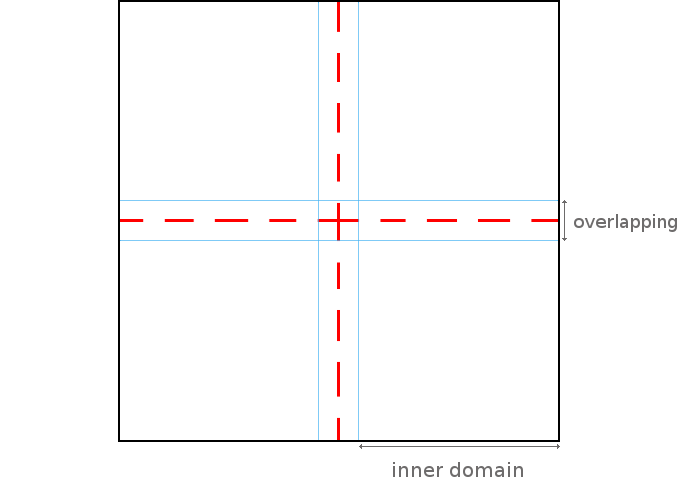
\includegraphics[scale=0.3]{figures/domain_overlap.png}
    \caption{\label{fig:overlap_domain}Représentation de l'overlapping - Domaine}
  \end{subfigure}%
  ~ 
  \begin{subfigure}[b]{0.5\textwidth}
    \centering
    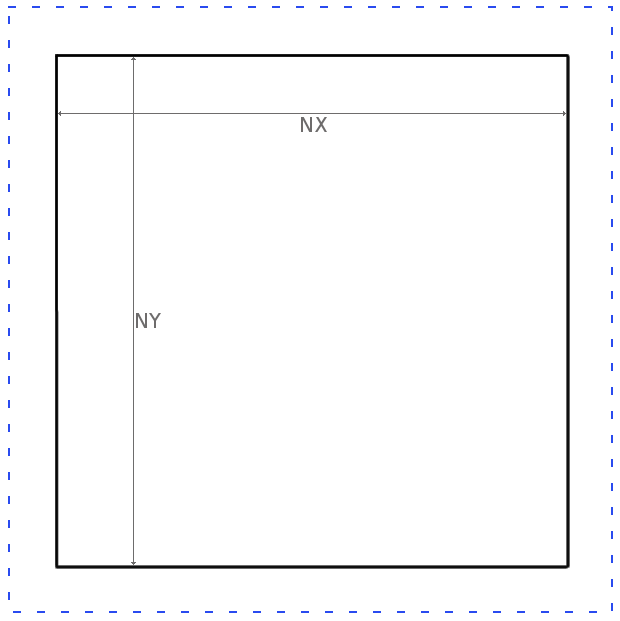
\includegraphics[scale=0.3]{figures/overlap.png}
    \caption{\label{fig:overlap_subdomain}Représentation de l'overlapping - Sous-domaine}
  \end{subfigure}
  \caption{\label{fig:overlap}Diffusion}
\end{figure}
% NX et NY représente la taille du domaine de validité d'un processus. Les pointillés bleus représente cet overlapping qui contiendra les valeurs des domaines adjacents.

L'exactitude des résultats dépendra donc de la taille de cet overlapping, c'est pour cela que le choix sera laissé à l'utilisateur même si une étude sera présenté.



\subsubsection{Méthode d'overlapping}
En pratique, il existe 2 méthode pour réaliser l'overlapping présenté précedemment, elles diffèrent seuleument dans le moment auquel les communications entre les processus seront réalisées. Mais l'idée générale reste la même. Les données permettant de calculer les gradients du sous-domaine d'un processus se trouvent sur ses processus voisins. On peut donc créer des ``cellules fantômes'' autour du sous-domaine qui contiendront les valeurs requises. Sur la figure \ref{fig:neighbor_buf}, on peut voir en orange les ``cellules fantômes'' qui recevront les valeurs voisines et en vert les valeurs qui seront envoyées aux processus voisins. 

\begin{figure}[h]
  \centering
  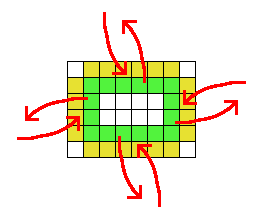
\includegraphics[scale=1]{figures/domain_overlap2.png}
  \caption{\label{fig:neighbor_buf}Motif de communication d'un processus}
\end{figure}


%\begin{figure}[h]
%  \centering
%  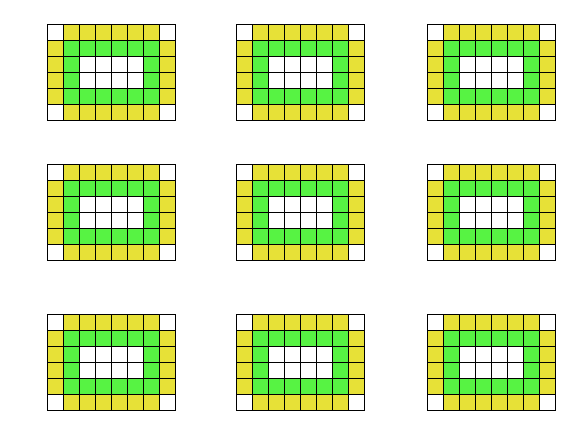
\includegraphics[scale=0.5]{figures/halo.png}
%  \caption{\label{fig:neighbor_buf} Motif de communication}
%\end{figure}

\paragraph{}Une méthode de Runge-Kutta est utilisée lors du calcul de l'avancé du temps. C'est une méthode d'analyse numérique permettant l'approximation de solutions d'équations différentielles. Elle est réalisé en 3 étapes (algo \ref{}) et dans chacune de ces étapes des gradients sont calculés.

\begin{algorithm}
  \caption{Time loop}
  \label{algo:time_loop}
  \begin{algorithmic}
     \FOR{time<final\_time} 
     \STATE {Call compute\_timestep} 
     \STATE {Call time\_step}
     \ENDFOR
  \end{algorithmic}
\end{algorithm}

\begin{algorithm}
  \caption{time\_step}
  \label{algo:time_step}
  \begin{algorithmic}
     \FOR{time<final\_time} 
     \STATE {Call RHS(1)} 
     \STATE {Call impose\_boundary\_conditions}
     \STATE {Call RHS(2)} 
     \STATE {Call impose\_boundary\_conditions}
     \STATE {Call RHS(3)} 
     \STATE {Call impose\_boundary\_conditions}
     \ENDFOR
  \end{algorithmic}
\end{algorithm}

\paragraph{1ère méthode}Cette première méthode consiste à réaliser les communications avant chaque appel à RHS. Ainsi, la région d'overlapping possède les valeurs calculées par les voisins et peuvent être utilisées pour les calculs locaux de gradient. Avec cette méthode, 3 grandes communications sont réalisées par pas de temps.

\paragraph{2éme méthode}Dans cette seconde méthode, un processus récupère les valeurs d'une seule variable conservative au moment du calcul du gradient correspondant. Cette fois-ci, les communicattions sont plus nombreuses et plus petites. 

%\paragraph{1ère méthode}Cette première méthode consiste à récupérer la région d'overlapping pour chaque variable conservative en début du pas de temps, avant tout calcul de gradient. L'évolution de ces points sera calculée et ils seront ensuite utilisés lors du calcul des gradients sur les différents champs. Avec cette méthode, une seule communication est réalisée par pas de temps mais le coût des calculs et du stockage est augmenté.


\paragraph{}J'ai donc ajouter ces méthodes au programme pour pouvoir comparer leurs performances respectives. La première méthode à l'avantage de reduiré la fréquence des communications en dupliquant des calculs sur plusieurs processus (augmentant donc le côut de ceux-ci).


\paragraph{}Dans la version séquentielle, un pas de temps maximal est calculé dans le but d'assurer la stabilité de l'algorithme. Ce calcul est donc dépendant de l'ensemble du domaine. Dans la version parallèle, chaque processus devra donc calculer le pas de temps maximal de son sous-domaine et le communiquer aux autres afin de trouver le pas de temps global (opération de réduction).

% \begin{itemize}
% \item pour le calcul du pas de temps; dans la version séquentielle, un pas de temps maximal est calculé dans le but d'assurer la stabilité de l'algorithme. Dans la version parallèle, chaque processeur devra donc calculer le pas de temps maximal de son sous-domaine et le communiquer aux autres afin de trouver le pas de temps global (opération de réduction).
% \item pour le calcul des gradients; une méthode compacte est utilisée pour calculer les gradients des différents champs. Une telle méthode implique que le gradient en un point est dépendante de tous les autres points du domaine. Il sera donc nécessaire d'échanger des informations entre les processus pour ce calcul reste juste.
% \end{itemize}



\subsection{Equilibrage de charge}
Lors d'un tel découpage de domaine, il est nécessaire de s'assurer que la quantité de travail réalisée par chaque processus est semblable à celle des autres. Le but est donc de distribuer le même nombre de mailles sur chaque processus. Dans le cas d'un domaine périodique ce problème n'apparaît pas car chaque processus possédent des regions d'overlapping dans toutes les directions. Cependant, si le domaine possède des frontières physique (cas symmétrique), certains sous-domaines n'auront pas le même besoin d'overlapping.

\paragraph{}Prenons l'exemple d'un domaine de 100x100x100 répartis sur une grille de 4x4x4 processus avec un overlapping de 4: si on découpe le domaine de manière triviale, on obtient donc 64 sous-domaines de taille 25x25x25. Si on ajoute ensuite les points d'overlapping, on retrouve 4 classes de sous-domaines ayant des tailles différentes (fig. \ref{fig:domain_desequilibre}); les coins du domaine auront donc 30x30x30 points, les autres sous-domaines situés sur les bordures physique auront 35x30x30 points, les sous-domaines situés sur les faces externes 35x35x30 et tous les autres 35x35x35. Comme on peut le constater dans le tableau \ref{arr:overlap_res}, la charge de calcul est désiquilibrée entre les processus et certain processus (ceux ayant le moins de travail) devront atteindre les autres pour les synchronisations présentées en début de partie. Même si ce comportement est moins marqué lorsque les sous-domaines sont plus grands (\ref{arr:overlap_res_big}), il est préférable de l'éviter.
  
Si on ajoute la taille totale de l'overlapping avant de découper le domaine, les tailles des domaines internes varient selon les processus mais la taille globale (domaine interne + overlapping) est identique. Toujours avec l'exemple précédent, si on ajoute la taille de l'overlapping à la taille globale, on obtient un domaine global de 124x124x124 points. On divise ensuite ce domaine entre les processus et on obtient cette fois-ci une seule classe de sous-domaines de 31x31x31 points. On joue ici sur la taille du domaine interne pour équilibrer la charge. Un sous-domaine se trouvant sur un coin aura un domaine interne de 27x27x27 alors qu'un sous-domaine de classe A aura 23x23x23 point sur son domaine interne.


\begin{figure}[ht]
  \centering
  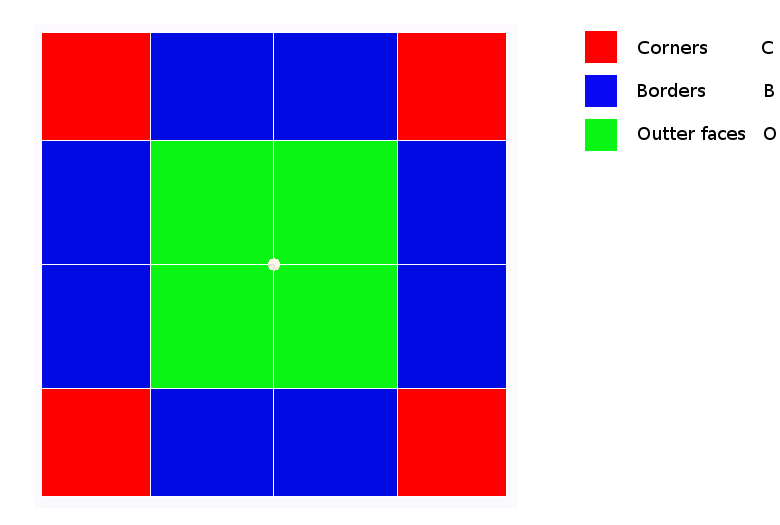
\includegraphics[scale=0.3]{figures/domain_dese.png}
  \caption{\label{fig:domain_desequilibre}Exemple de déséquilibre de charge}
\end{figure}

\begin{table}[h]
  \begin{center}
    \begin{tabular}{|P{2cm}|P{3.5cm}|P{3.5cm}|}
      \hline
      & Taille & Overhead \\ \hline
      C & 29x29x29 & 0\%  \\ \hline
      B & 33x29x29 & 13.8\%  \\ \hline
      F & 33x33x29 & 29.5\%  \\ \hline
      A & 33x33x33 & 47.3\%  \\ \hline      
    \end{tabular}
    \caption{\label{arr:overlap_res}Surcout de calcul - 100x100x100, 64 processus, overlapping 4}
  \end{center}
\end{table}


\begin{table}[h]
  \begin{center}
    \begin{tabular}{|P{2cm}|P{3.5cm}|P{3.5cm}|}
      \hline
      & Taille & Overhead \\ \hline
      C & 205x205x205 & 0\%    \\ \hline
      B & 210x205x205 & 2.4\%  \\ \hline
      F & 210x210x205 & 4.9\%  \\ \hline
      A & 210x210x210 & 7.5\%  \\ \hline      
    \end{tabular}
    \caption{\label{arr:overlap_res_big}Surcout de calcul - 1000x1000x1000, 125 processus, overlapping 5}
  \end{center}
\end{table}


\paragraph{}Un déséquilibre de charge peut également apparaître lors de la phase d'initialisation, même si son impact est failble, il est préférable de l'éviter. En effet, il faut éviter qu'un seul processus doive initialiser l'ensemble du domaine puis envoyer les informations calculées à tous les autres processus. Dans le cas de ce programme l'initialisation peut-être réalisée de manière indépendante (sans aucune synchronisaton). En effet, les initialisations simples (valeur d'une variable fournies dans le fichier de configuration) ne nécessite aucun calcul. Les initialisation nécessitant des calculs sont en général basée sur la position physique des point du domaines et peuvent donc être initialisés en totale indépendances, le plus souvent par une fonction.

\subsection{Communications}Je m'intéresse ici aux méthodes de communications utilisées dans la première méthode présentée ci-dessus. En effet la seconde méthode d'overlapping n'induit qu'au plus 2 communications par processus par calcul de gradients et ne pose donc pas de problèmes particuliers. En revanche, pour la première méthode il faut effectuer au plus 2x3 communications par appel à la fonction update. J'ai testé plusieurs de communications pour comparer leurs performance. J'ai dans un premier temps utilisé la fonction MPI\_Neighbor\_alltoallv. Pour l'utiliser, il faut préparer un buffer qui contiendra les données à envoyer à chacun de ses voisins(fig. \ref{fig:neighbor_pos}). La fonction s'occupe elle-même d'envoyer la bonne partie du buffer au bon voisin selon leur disposition sur la grille cartésienne. Après l'appel à cette fonction, le buffer de réception contient les données de tous les voisins autour d'un processus. Il ne reste plus qu'à stocker les variables reçues à leur place. 

\begin{figure}[h!]
  \centering
  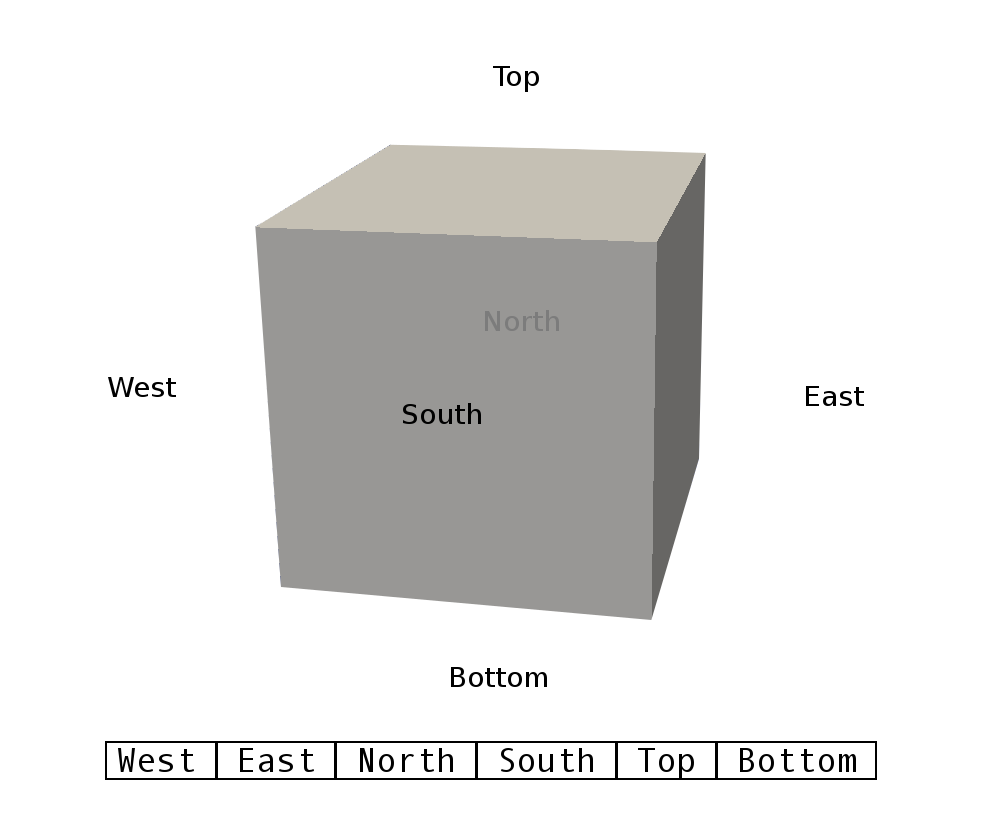
\includegraphics[scale=0.3]{figures/neighbor_pos.png}
  \caption{\label{fig:neighbor_pos}Positions des valeurs des voisins}
\end{figure}

\paragraph{}Cependant cette fonction est relativement récente et peut ne pas être disponible sur certain calculateur qui seront utilisé. Il m'a donc été demandé d'implémenter une seconde méthode dans un soucis de portabilité. C'est une implémentation triviale de la fonction MPI\_Neighbor\_alltoallv; on parcourt les dimensions du domaines, et pour chaque dimensions, on effectue 2 envois et 2 réceptions.

\paragraph{}Le coût d'une telle méthode ne se résume donc pas simplement aux coûts de communications mais aussi aux nombreuses copies réalisées pour créer le buffer d'envoi et pour ``eclater'' le buffer de reception. Ce coût sera donc étudié dans la partie suivante.

\subsection{Validation}

\paragraph{Cas d'un unique processus}Avant de tester la validité du programme avec plusieurs processus, il est nécessaire de s'assurer qu'il peut être lancé avec un seul processus et que les résulats fournis soient exactement identiques à la version 3D validée à la section \ref{sec:3D-validation}. Même si ce test paraît trivial, il est important de le faire. Il sera également utile de comparer le temps pris par ce test par rapport au temps de la version 3D séquentielle pour estimer le surcôut pouvant être induit par l'utilisation de MPI (découpage du domaine, calcul de l'overlapping, fausses communications ...).

\paragraph{Cas avec décomposition de domaine}
Comme vu dans la section \ref{sec:p2-tr} le calcul des gradients est dépendant de l'ensemble du domaine. Pour s'assurer de l'exactitude des résultats obtenus dans cette version MPI, j'ai donc utiliser un overlapping assez grand permettant d'affiner les résultats au maximum. J'ai ensuite calculer les valeurs moyennes des champs de la solution afin de les comparer avec ceux obtenus avec la version séquentielle du programme (\ref{sec:3D-validation}).

\begin{table}[h]
  \begin{center}
    \begin{tabular}{|c|c|c||c|c|c|c||c|c|c|}
      \hline
      Overlap & 12 & 11 \\
      \hline
      Mean error & 10E-14 & 10E-10 \\
      \hline
    
    \end{tabular}
    \caption{\label{arr:overlap_res} Résultats obtenus}
  \end{center}
\end{table}
